\documentclass[a4paper,12pt]{scrartcl}
\usepackage[utf8]{inputenc}
\usepackage[plainheadsepline]{scrpage2}
\usepackage[margin=2cm]{geometry}
\usepackage{fontenc}
\usepackage{marvosym}
\usepackage{lastpage}
\usepackage{amsmath, enumerate, amssymb}
\usepackage{graphicx}
\usepackage{listings}
\usepackage{dsfont}
\setlength{\footskip}{1cm}
\setheadsepline{1pt}

\setlength{\parindent}{0pt}
\allowdisplaybreaks[1]

\renewcommand*{\headfont}{\normalfont}

\begin{document}
\section{Intervallbaum-Index}
\textbf{1. Intervalle einfügen:}\\
Das Intervall muss im Baum an der richtigen Stelle eingefügt werden und der Baum muss gegebenenfalls neu balanciert werden (z.B. wie ein AVL-Baum).\\\\
Bsp.: Einfügen des Intervalls [12,15]\\\\
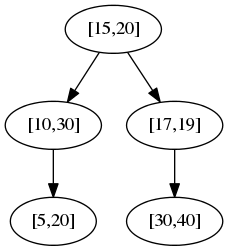
\includegraphics[width=0.2\textwidth]{1.png}$~~~~~~~~~~~$
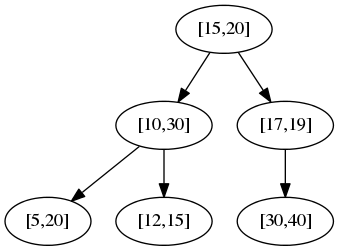
\includegraphics[width=0.3\textwidth]{2.png}\\\\
\textbf{2. Intervall mit Startpunkt $>$ Endpunkt einfügen:}\\
Wenn ein Intervall (S,E) mit S$>$E eingefügt wird, dann sollte unser Programm eine Fehlermeldung ausgeben und darauf hinweisen, dass die Grenzen für das Intervall nicht korrekt sind.\\\\
Bsp.: Einfügen des Intervalls [20,10] in einen beliebigen Baum.\\\\
\textbf{3. Intervall mit Start- bzw. Endpunkt außerhalb des betrachteten Zahlenbereichs:}\\
Wenn ein Intervall in dem Baum eingefügt werden soll, das teilweise oder vollständig außerhalb unseres Zahlenbereichs liegt (Länge des Genoms), dann muss es eine Fehlermeldung geben, die dem Nutzer mitteilt, dass der gültige Zahlenbereich überschritten wurde.\\\\
Bsp.: Einfügen des Intervalls [-5,7] in einen beliebigen Baum.\\\\
\textbf{4. Schon vorhandenes Intervall einfügen:}\\
Duplikate sollen von unserem Baum nicht gespeichert werden, d.h. es wird kein neuer Knoten hinzugefügt, sondern die Informationen (bei uns also Pointer auf Dateien) des neuen Knotens müssen im bereits vorhandenen Knoten mitgespeichert werden.\\\\
Bsp.: Einfügen des Intervalls [15,20] in den folgenden Baum\\\\
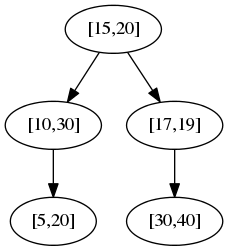
\includegraphics[width=0.2\textwidth]{1.png}\\\\\newpage
\textbf{5. Suche nach vorhandenem Intervall:}\\
Bei der Suche sollen alle Intervalle ausgegeben werden, die das gesuchte Intervall in irgendeinem Punkt überlappen.\\\\
Bsp.: Suche im folgenden Baum\\\\
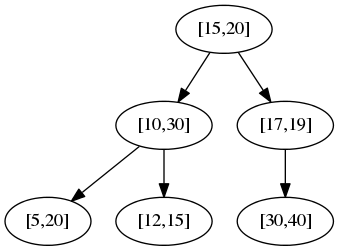
\includegraphics[width=0.3\textwidth]{2.png}\\\\Suche [4,5] $\Rightarrow$ gib [5,20] aus\\
Suche [25,35] $\Rightarrow$ gib [10,30] und [30,40] aus\\
Suche [20,20] $\Rightarrow$ gib [15,20] und [5,20] aus

\section{QueryReceiver}
\subsection{Testfall 1 - erfolgreiche Intervallanfrage ohne Metadaten}
\begin{verbatim}
  Eingabe
{
  "source": The Cancer Atlas,\usepackage[utf8]{inputenc}
  "chromosome": 3,
  "position": {"from": 100, "to": 200},
  "zoom": 1,
  "subindex": ,
  "hasDetail": (false)
}

  Ausgabe
{
  {
    "source:" The Cancer Atlas,
    "chromosome": 3,
    "position": {"from": 100, "to": 200},
    "details": { "refseq": ,
                "mutations": [{ "name": ,
                                "position": {"from": , "to": },
                                "metadata":
                              },]},
    "graph": {
              { "subintervall": Anzahl der Subintervalle,
                "counts": Anzahl der Ergebnisse
              }
            }
  }
}
\end{verbatim}

\subsection{Testfall 2 - erfolgreiche Intervallanfrage mit Metadaten}
\begin{verbatim}
  Eingabe
{
  "source": The Cancer Atlas,
  "chromosome": 3,
  "position": {"from": 100, "to": 200},
  "zoom": 1,
  "subindex": ,
  "hasDetail": (true)
}

  Ausgabe
{
  {
    "source:" The Cancer Atlas,
    "chromosome": 3,
    "position": {"from": 100, "to": 200},
    "details": { "refseq": Referenzsequenz,
                "mutations": [{Mutation1},{Mutation2},...]},
    "graph": {
              { "subintervall": ,
                "counts":
              }
            }
  }
}
\end{verbatim}

\subsection{Testfall 3 - erfolglose Intervallanfrage}
\begin{verbatim}
  Eingabe
{
  "source": The Cancer Atlas,
  "chromosome": 3,
  "position": {"from": 100, "to": 200},
  "zoom": 1,
  "subindex": ,
  "hasDetail": (true)
}

  Ausgabe
{
  {
    "source:" The Cancer Atlas,
    "chromosome": 3,
    "position": {"from": 100, "to": 200},
    "details": { "refseq": ,
                "mutations": ...},
    "graph": {
              { "subintervall": ,
                "counts":
              }
            }
  }
}
\end{verbatim}

\subsection{Testfall 4 - erfolgreiche Namensanfrage}
\begin{verbatim}
  Eingabe
{
  "source": The Cancer Atlas,
  "chromosome": 3,
  "search": "Gen im Cancer Atlas"
}

  Ausgabe
{
  "source": The Cancer Atlas,
  "chromosome": 3,
  "search": "Gen im Cancer Atlas",
  "position": {"from": Startposition, "to": Endposition}
}
\end{verbatim}

\subsection{Testfall 5 - erfolglose Namensanfrage}
\begin{verbatim}
  Eingabe
{
  "source": The Cancer Atlas,
  "chromosome": 3,
  "search": "Gen, dass nicht im Cancer Atlas ist"
}

  Ausgabe
{
  "source": The Cancer Atlas,
  "chromosome": 3,
  "search": "Gen im Cancer Atlas",
  "position": " "
}
\end{verbatim}

\subsection{Testfall 6 - fehlerhafte Anfrage}
\begin{verbatim}
  Eingabe
{
  "source": ""
}

  Ausgabe
{
  "answer": "unknown format"
}
\end{verbatim}
\end{document}